\subsection{Classifier Performance}
\label{sec:constraintdetection}

Our first experiment evaluates how model and prompt design affect constraint classification. We derive four variants of the prompt in Figure~\ref{fig:classifyprompt} by enabling or disabling \emph{examples} and \emph{table context} (\emph{No Context}, \emph{Table Context}, \emph{Examples}, \emph{Examples + Table Context}) and evaluate them with six LLMs on all datasets (Figure~\ref{fig:classifier-results}). Because sentences missed here cannot be recovered by the mapper, we require recall $\geq 0.90$ on every dataset when selecting a default configuration.

\begin{figure}[!ht]
    \centering
    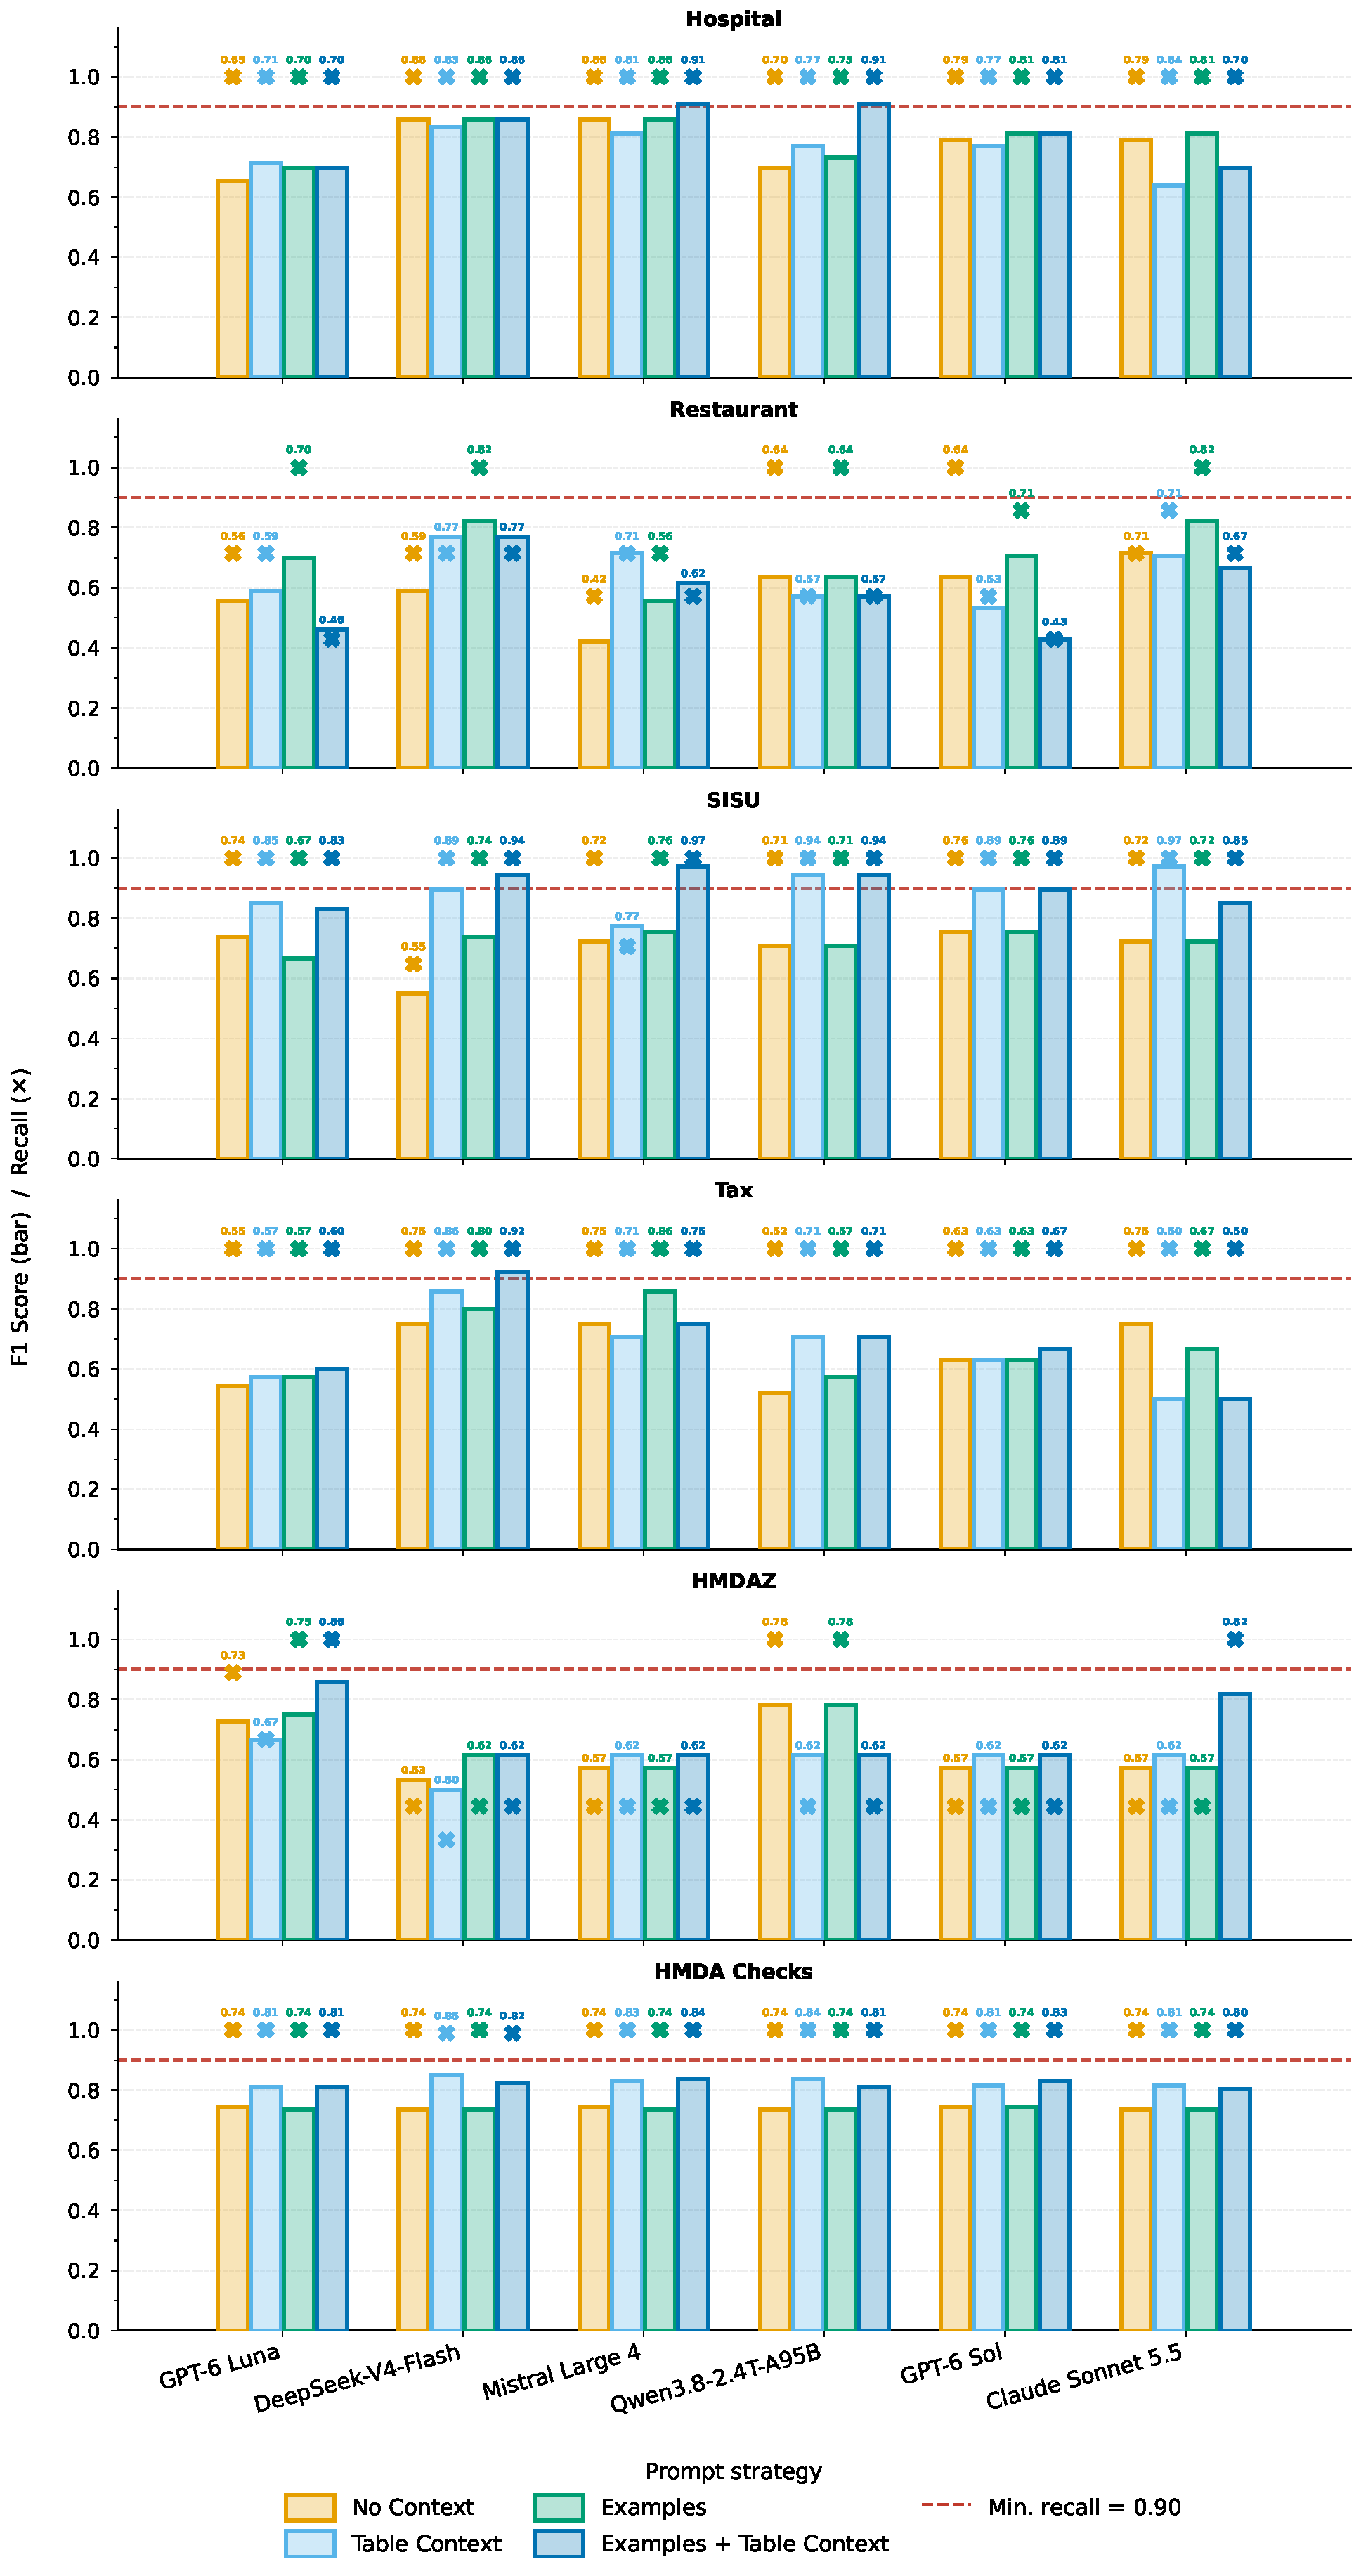
\includegraphics[width=\columnwidth]{figures/results/v3_fig6_classifiers.pdf}
\caption{Constraint classification F$_1$ (bars) and recall (\textsf{x}) across models and prompt variants. The dashed line marks the 0.90 recall threshold.}
    \label{fig:classifier-results}
\end{figure}

On Hospital, Tax, SISU, and HMDA Checks, almost every configuration reaches recall 1.00, so differences lie in precision. On HMDAZ and Restaurant, recall is the bottleneck: on HMDAZ, most configurations recover only 4 of the 9 constraint sentences, missing regulatory definitions (e.g., when a mortgage is high-cost) that read as scope statements, although each implies a checkable condition. Only three configurations satisfy this recall requirement on all six datasets: \emph{Qwen3.8-2.4T-A95B} with \emph{Examples} (mean F$_1$ 0.69), \emph{GPT-6 Luna} with \emph{Examples} (0.69), and \emph{Qwen3.8-2.4T-A95B} with \emph{No Context} (0.68); we select the first. Configurations with higher mean F$_1$ exist (e.g., DeepSeek-V4-Flash with \emph{Examples + Table Context}, 0.82), but they miss more than half of the HMDAZ constraints.

Table context has two opposite effects. It is the only signal that raises precision on HMDA Checks, where non-constraint edits are phrased like checkable ones but refer to aggregates or external data: without it, F$_1$ equals that of the all-positive classifier (0.74); with it, 0.80--0.85. On wide schemas, however, it does not help recall: on HMDAZ (135 columns), 9 of the 12 table-context configurations stay at or below 0.44. Averaged over models and datasets, \emph{Examples} gives the best recall (0.93), and table context higher precision (0.71 vs.\ 0.58--0.62) at lower recall (0.85--0.87).
Without examples or context, classification is already strong on the controlled datasets (recall 1.00, mean F$_1$ 0.72 on Tax and Hospital), and the best variant adds only 0.04. On SISU, Restaurant, and the HMDA datasets, the gain is larger (0.66 to 0.75 with \emph{Examples + Table Context}), mostly through precision. A plausible explanation is that LLM-written sentences resemble text these models produce or saw in pretraining; we cannot verify such exposure, but context matters most on real regulatory text.
